\chapter{Hluboké Q-učení}

\section{Základní princip}
\subsection{Neuronová síť}
Než se dostaneme k hlubokému q-učení, budeme se nejprve muset seznámit s pojmy neuronová síť a q-učení. Začněme tedy s neurovnovými sítěmi.
Abychom si mohli říct, co neurovnové sítě jsou, musíme se nějdřív seznámit s její základní jednotku - perceptron.
\par
Perceptron je algoritmus, který má na vstupu několik hodnot $x_i$ a jeden výstup. S každou vstupní hodnotou je spojena jedna váha $w_i$.
Kromě váh vstupů obsahuje perceptron ještě tzv. práh. Perceptron spočítá vážený součet vstupů a porovná výsledek s prahem. Pokud je výsledek větší než práh, tak perceptron vrací hodnotu 1, jinak 0.
Můžeme zde ale využít triku pro zbavení se prahu. K práhu můžeme přistupovat jako k další váze s konstantním vstupem -1.
V takovém případě pak perceptron provádí porovnání váženého součtu vstupů s hodnotou 0. 
\newline
Matematicky zapsáno:
\[f(\sum_{i=0}^{n} w_if_i)\], kde $f$ vrací 1 pro $x>0$ a 0 jinak.

Trénování daného perceptronu probíhá pomocí předkládání dvojic vstupů a výstupů $(x,y)$ z trénovací množiny a upravování váh následujícím způsobem:
\newline
\[w_i = w_i + r(y-f(x_i)x_i\], kde $r$ je parametr učení.

Rozhodovací hranice perceptronu představuje nadrovinu ve vstupním prostoru. Lze ukázat, že trénování perceptronu zkonverguje, pokud jsou třídy v datech lineárně separabilní.

Většinou ale řešíme problémy, kde třídy v datech lineárně separabilní nejsou, v takových případech nám jeden perceptron nestačí a potřebujeme jich využít víc.
Spojením více perceptronů získáváme dopřednou neuronovou síť. Ta se skládá z vrstev perceptronů, kde vstupy perceptronů první jsou samotná data $x$ a vstupy perceptronů v dalších vrstávch jsou rovny výstupům perceptronů z vrstvy předchozí.

Pro trénování více vrstvých perceptronů se používá gradientní metoda. Z toho důvodů se využívají jiné funkce $f$, než ta zmíněná nahoře, ta má totiž gradient ve většíně případů roven 0.
Typickým příkladem používané funkce je sigmoid \[f(x) = \frac{1}{1+e^{-x}}\].

Následně musíme zvolit chybovou funkci $L(x,y|w)$ neuronové sítě. Zde se typicky využívá střední kvadratická chyba (ang. Mean squared error).
Chybová funkce se zderivuje podle vah v síti a následně se jednotlivé váhy upraví.
\newline
\[w_i = w_i + \alpha\frac{\partial L(x,y|w)}{\partial w_i}\]

\url{https://ocw.mit.edu/courses/health-sciences-and-technology/hst-947-medical-artificial-intelligence-spring-2005/lecture-notes/ch7_mach3.pdf}
\todo{strana 9 až 13}

\subsection{Zpětnovazební učení}
Podobně jako v předchozí sekci, i zde musíme nejprve zavést nové pojem a terminologii, než budeme moci říct, co je cílem zpětnovazebního učení.
Popišme si nejprve, co je to markovský rozhodovací prostor.
Markovský rozhodovací prostor popisuje prostředí a je definován čtveřicí $(S,A,P,R)$, kde $S$ je množina stavů, $A$ je množina všech akcí (případně $A_s$ představuje množinu akcí, které mohou být provedeny ve stavu $s$), 
$P: S \times A \times S \rightarrow [0,1]$ představuje přechodovou funkci, 
kde $P_a(s,s')$ vrací pravděpodobnost, že se aplikováním akce $a$ ve stavu $s$ dostaneme do stavu $s'$, 
a $R: S \times A \times S \rightarrow \mathbb{R}$ představuje funkci odměn $R_a(s,s')$, která vrací odměnu, kterou agent obdrží, pokud ve stavu $s$ provede akci $a$ a dostane se tak do stavu $s'$.
Přechodová funkce i funkce odměn musí navíc splňovat podmínku, že musí být jejich hodnoty nezávislé na předchozích stavech.

\url{https://ocw.mit.edu/courses/aeronautics-and-astronautics/16-410-principles-of-autonomy-and-decision-making-fall-2010/lecture-notes/MIT16_410F10_lec22.pdf}

Chování agenta v prostředí můžeme popsat pomocí strategie $\pi: S \times A \rightarrow [0,1]$, ta určuje pravděpodobnost, že se agent ve stavu $s$ rozhodne pro akci $a$.
Pro agenta v prostředí ještě definujme jeho celkovou odměnu jako \[\sum_{t=0}^{\infty} \gamma^tR_{a_t}(s_t,s_{t+1})\], kde $\gamma<1$ je diskontní faktor, díky kterému je suma konečná a $a_t$ je akce agenta vybraná v kroku t.
Cílem zpětnovazebního učení je nalézt optimální strategii $\pi^\star$, kde $a_t=\pi^\star(s_t)$, takovou, že její celková odměna je maximální.

Hodnotu stavu $s$ při použití strategie $\pi$ lze definovat jako 
\newline
\[V^{\pi}(s)=[\sum_{t=o}^{\infty} \gamma^tr_t|s_0=s]\], kde $r_t$ značí odměnu získanou v kroku t.
Podobně také můžeme definovat hodnotu $Q^{\pi}(s,a)$ akce $a$ provedené ve stavu $s$ při následování strategie $\pi$.
\[Q^\pi(s,a)=\sum_{s'}P_a(s,s')[R_a(s,s') + \gamma\sum_{a'} \pi(s',a')Q^\pi(s',a')]\]
Z Bellmanovy rovnice pro optimální strategie platí:
\[Q^*(s,a)=R_a(s,s') + \gamma\max_{a'}Q_k(s',a')\]

Agent ke zlepšování své strategie může využívat přechodové funkce a funkce odměn. Často ale agent hodnoty jednotlivých stavů předem nezná a musí se je učit za běhu.
Zároveň musí volit mezi explorací tj. prohledávání prostoru a exploatací tj. využívání známého. Zde využijeme $\epsilon$-hladového (ang. $\epsilon$-greedy) přístupu, kdy s pravděpodobností $\epsilon$ vybere náhodou akci a s pravděpodobností $1-\epsilon$ vybere nejlepší známou akci.

Nyní se už dostáváme ke Q-učení. $Q$ je reprezentována jako matice zpočátku inicializovaná samými nulami. Agent následně ve stavu $s_t$ vybírá například $\epsilon$-hladovým přístupem akci $a_t$, získá od prostředí odměnu $r_t$ a přesune se do stavu $s'$.
Na základě těchto informací se provede aktualizace matice následovně:
\newline
\[Q(s_t,a_t) \leftarrow (1-\alpha)Q(s_t,a_t) + \alpha(r_t + \gamma(\max_a(Q(s_{t+1},a))))\]


\subsection{Hluboké q-učení}
Po seznámí se základy neuronových sítí a zpětnovazebního učení můžeme přejít k hlubokému Q-učení.
Hluboké Q-učení následuje stejnou myšlenku jako obyčejné Q-učení, také chceme nalézt odměnu vybrané akce v současném stavu stavu.
Hlavním rozdílem oproti normálnímu Q-učení je způsob jak se Q hodnoty reprezentují. V normálním Q-učení jsou Q hodnoty uložené v matici, ta může být v případě velkých prostorů příliš obrovská a Q-učení pak může probíhat velmi pomalu, nebo dokonce vůbec.
V Hlubokém Q-učení bude Q reprezentováno pomocí neuronové sítě.

Trénování se provádí pomocí porovnání rozdílu aktuální odměny $R_a(s,s')$ prostředí od odměny spočítané pomocí Bellmanovy rovnice z Q.
Cílem je tedy minimalizovat rozdíl mezi \[Q(s,a) \hspace{5mm}\text{a}\hspace{5mm}  R_a(s,s') + \gamma\max_{a'}Q_{\theta}(s',a')\], kde $Q_{\theta}$ jsou parametry neurovnové sítě reprezentující matici Q.
Chybovou funkcí pro trénování neuronové sítě pak může být střední čtvercová chyba tohoto rozdílu.

\section{Aplikace}
V praxi bylo hluboké Q-učení použito například pro naučení se hraní atari her. 
\url{https://www.cs.toronto.edu/~vmnih/docs/dqn.pdf}

Namísto ručně zpracovaných informacích o stavu hry zde byly jako vstupy využity přímo vizuální výstupy hry.
Q-síť je proto reprezentována konvoluční neuronovou sítí, která na vstupu bere vektor pixelů obrázku hry a na výstupu vrací odhad budoucích odměn pro každou z možných akcí.
Modelu nebylo řečeno nic o principu fungování hry. Model se učil pouze na základě vizuálního výstupu, odměn, které dostával od prostředí, konečných stavů a množiny možných akcí, tedy stejným přístupem, jak by ke hře přistupoval člověk.

Stejná neuronová síť byla použitá na sedmi různých atari hrách. Na šesti z nich překonala všechny stávající přístupy, které využívaly algoritmy zpětnovazebního učení a na třech z nich překonala výsledky nejlepších lidských hráčů.



\section{Aplikace}
\subsection{Úvod}
Herní prostředí nám v každém kroku vrací odměnu, kterou oba z hráčů za jejich akci obdrželi. Tuto informaci jsme v experimentech provedených v rámci genetického programování, nevyužili, ale zde budou hrát velkou roli.
Za každý krok, kdy hra ještě neskončila získávají agenti automaticky odměnu 1. Na konci hry agent obdrží vysokou odměnu v případě výhry a v případě prohry naopak získá penalizaci v podobě odměnu vysoké záporné hodnoty. Tyto hodnoty se pro jednotlivé experimenty mírně liší.
Odměnu za výhru, nebo prohru získá agent až na úplném konci hry, to může ztěžovat učící proces. Proto prostředí dává agentům i průběžné menší odměny, pro lepší možnost učení se.

Konkrétně to jsou následující odměny:
\begin{itemize}
    \item Sestřelení asteroidu
        \newline
        Za každý sestřelený asteroid získává agent odměnu hodnoty 5.
    \item Zasažení asteroidem nepřátelské vesmírné lodi
        \newline
        Zranění nepřítele je právě to, co agent potřebuje pro přiblížění se vítězství, proto za každé takové zasažení získává od prostředí odměnu v hodnotě 20.
    \item Zasažení asteroidem vlastní vesmírné lodi
        \newline
        Takový stav je pro agenta znevýhodňující a cílem je se mu vyvarovat, proto za takovýto stav agent od prostředí dostává penalizaci v hodnotě -10.
\end{itemize}


\todo{presunout do kapitoly o deep q}
V rámci učení agentů budeme využívat epsilon-hladového (ang. epsilon-greedy) přístupu. V každém kroku q-učení volíme další akci a epsilon-hladový přístup nám v tom pomáhá následovně.
Vygenerujeme náhodnou hodnotou z intervalu $(0,1)$ a pokud je tato hodnota menší než hodnota epsilon, tak provedeme volbu akce náhodně, v opačném případě volíme nejlepší akce dle q-sítě.
Hodnota epsilon se na počátku inicializuje na hodnotu 1 a po každé zahrané hře se sníží vynásobením koeficientem menším než 1. 
Epsilon-hladový přístup způsobuje, že z počátku učení se zkoušejí náhodné akce a v průběhu přechází ze zkoušení nových akcí do prohledávání již osvědčených akcí.

\todo{presunout do kapitoly o deep q}
\par
Při trénování se nám stává, že měníme funkci, která odhaduje Q a tím je ovlivněno i chování agenta a odhady. K zachování větší stability trénování využijeme konceptu přehrávání zkušeností (ang. Experience replay).
Při hraní hry si v každém kroku ukládáme do paměti pětici současného stavu, provedené akce, obdržené odměny, stavu, do kterého jsme se dostali a informace zda hra neskončila.
Po konci zahrání hry následně náhodně vybíráme tyto pětice z paměti a trénování provádíme na nich.






\subsection{Experiment 4: Soupeření s obranným agentem}
V 1. experimentu jsme za pomocí genetického programování hledali agenta, který je úspěšný v souboji s obranným jedincem. Pro určení jak agent v souboji obstál jsme využívali fitness funkci.
Zde, pomocí hlubokého q učení, budeme také učit agenta vzájemnými souboji s obranným agentem, ale budeme namísto fitness funkce používat pro trénování odměny.

S 1. experimentem zde bude také stejný přístup ke vstupům a výstupům. 
Na vstupu budou opět délky všech čtyř akčních plánů a počet kroků před srážkou vesmírné lodi s asteroidem.
A na výstupu čtyři hodnoty reprezentující výběr konkrétního akčního plánu.

Q učení spočívá v učení se rozhodování akcí. Akce zde v tomto pojetí však nebudou elementární akce, nýbrž akční plány. 
Q-síť bude tedy volit akční plány a proto zde budeme muset provádět mezikrok pro přechod od akčních plánů k akcím.
Nejprve vždy zvolíme akční plán a následně pro pokračování v simulaci hry z vybraného akčního plánu vybereme první akci.
V tomto experimentu budeme využívat přehrávání zkušeností, tj. budeme průběžně ukládat informace o přechodech do dalších stavů. 
I Zde, pro zapamatování si zkušenosti, platí, že akcí budeme rozumět akční plán.


Parametry experimentu:
\begin{itemize}
    \item Na konci hry agent obdrží agent odměnu v hodnotě 2000 v případě výhry a -1000 v případě prohry.
    \item Q-síť je hustá neuronová síť s pěti vstupy, čtyřmi výstupy a jednou skrytou vrstvou. 
    \item Během učení bude zahráno 1500 her.
    \item Konstanta pro snižování epsilon je nastavena na 0.998. To znamená, že například po zahrání 1400 her se bude v další hře volit akce náhodně jen v 6\% případů. 
\end{itemize}

\par
V souboji s obranným agentem se výslednému agentovi podařilo zvítězil pouze ve čtyřech hrách. 
Nepodařilo se nám tedy sice nalézt agenta, který by porážel obranného agenta, ale dosáhli jsme jiného zajímavého výsledku.
Velkým přínosem tohoto experimentu je pestrá strategie nalezeného agenta. Výsledný agent ve velkém zastoupení používá všechny akční plány (viz \ref{Výsledek experimentu 04}). 
Výsledkem je agent, který se brání nejen sestřelováním nepřátelskqých asteroidů, ale i vyhýbáním se. A díky tomu se agent také pohybuje a nezůstává staticky stát na stejném místě po celou dobu hry.
Toho se nám také podařilo dosáhnout ve 3. experimentu, ale srovnání s agentem získaným ze 3. experimentu je tento agent daleko více obranyschopný.




\begin{figure}[p]\centering
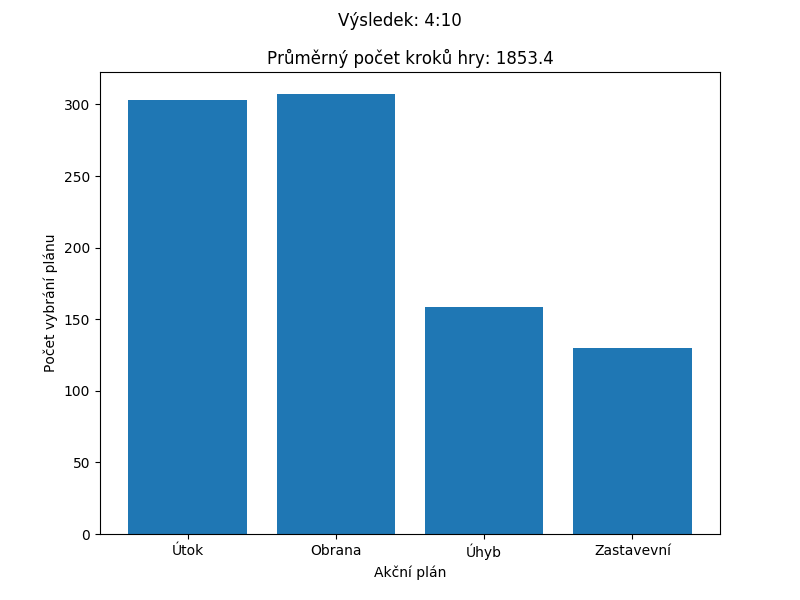
\includegraphics[width=145mm, height=110mm]{./Obrazky/Experiment04Results.png}
\caption{Výsledek experimentu 4}
\label{Výsledek experimentu 04}
\end{figure}

\subsection{Experiment 5: Soupeření s obranným agentem - Rozšířeno}
V předchozím experimentu jsme dosáhli zajímavého chování agenta, ale nepodařilo se nám stabilně vyhrávat nad obranným agentem.
Zkusíme proto předchozí experiment rozšířit. 
V tomto experimentu zkusíme přidat další vstupní argumenty, které by mohli agentovi pomoct v rozhodování.

Přidané parametry:
\begin{itemize}
    \item Dvojice počtu zbývajících životů obou agentů            
    \item Počet nebezepčných asteroidů v blízké vzdálenosti od agenta
    \item Celkový současný počet nebezpečných asteroidů v celé hře
\end{itemize}
Snaha všech přidaných argumentů je rozšířit agentovi poznání o současném stavu hry a díky tomu dát agentovi možnost se komplexněji rozhodovat pro akční plány.

Parametry experimentu:
\begin{itemize}
    \item Odměny za finální stav hry zůstávají stejné. Na konci hry agent obdrží agent odměnu v hodnotě 2000 v případě výhry a -1000 v případě prohry.
    \item Q-síť je stejná síť jako v předchozím případě, jen namísto pěti vstupních argumentů, bude nyní přijímat vstupů devět.
    \item V tomto experimentu zkusíme kvůli rozšíření vstupních argumentů také prodloužit trénování sítě, proto bude v rámci trénování zahráno 3000 her.
    \item Adekvátně ke zvýšení počtu zahraných her také zvětšíme konstantu pro snižování epsilon z hodnoty 0.998 na 0.9989. Díky tomu bude stejné pravděpodobnosti 6\% pro volbu náhodné akce dosaženo přibližně po zahrání 2550 her.
\end{itemize}

\begin{figure}[p]\centering
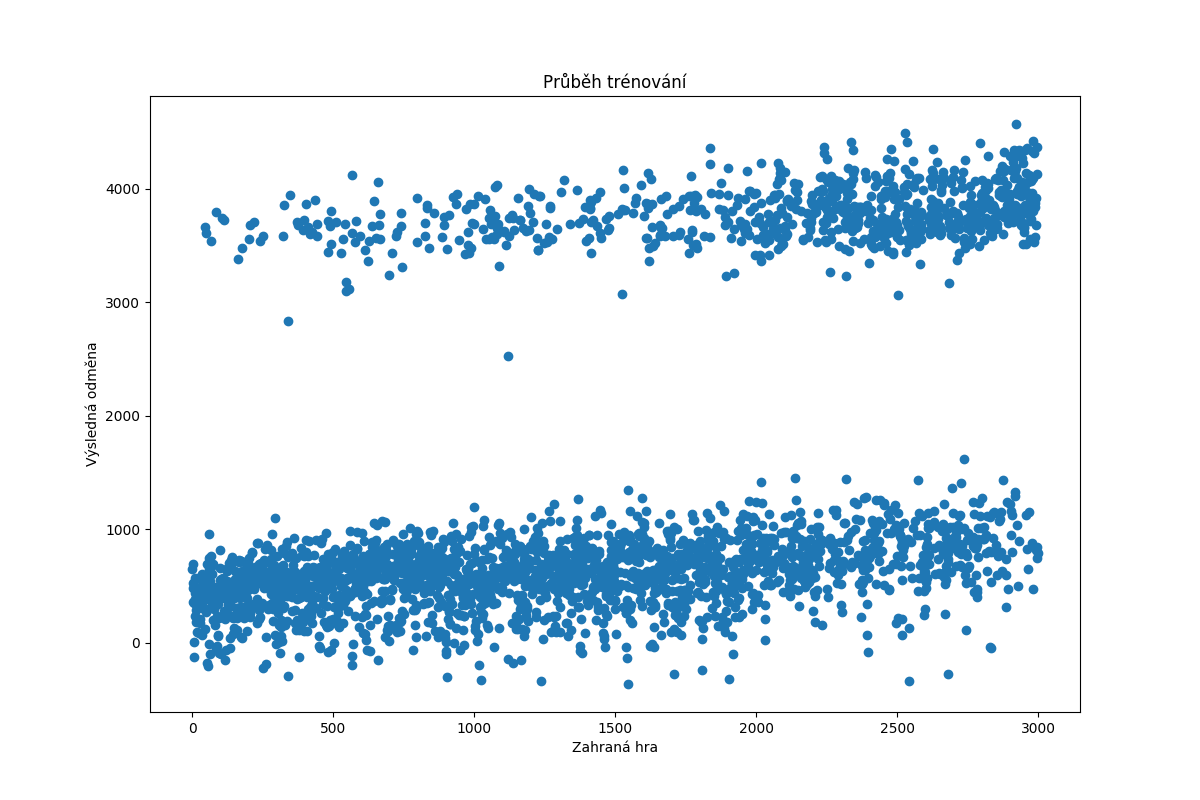
\includegraphics[width=145mm, height=110mm]{./Obrazky/Experiment05Training.png}
\caption{Průběh trénování v experimentu 5 - Výsledné odměny jsou součtem počtu kroků hry a odměny (resp. penalizace) za výhru (resp. prohru). Samotné tyto odměny tvoří rozdíl v hodnotě 3000, díky tomu je z obrázku zřetelné, ve kterých hrách agent vyhrál.}
\label{Průběh trénování experimentu 06}
\end{figure}




\begin{figure}[p]\centering
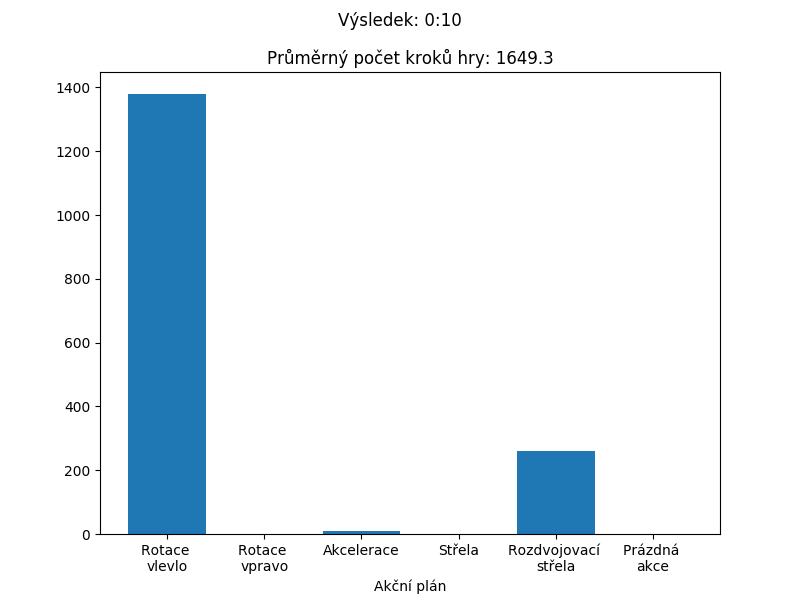
\includegraphics[width=145mm, height=110mm]{./Obrazky/Experiment05Results.png}
\caption{Výsledek experimentu 5}
\label{Průběh trénování experimentu 06}
\end{figure}


Výsledný agent dopadlo velmi úspěšně. Z průběhu trénování vidíme, že agent se velmi dobře učil a od přibližně 2300. hry (viz \ref{Průběh trénování experimentu 06}) už začal vyhrávat ve větší části her.
Rozšířením vstupních argumentů a přidání trénovacích her se nám podařilo zlepšit výsledek z předchozícho experimentu.
Agent sice ztratil pestrost akčních plánů, ale za to se významně zlepšil ve vyhrávání. Z výsledku 4:10 z předchozícho experimentu se zlepšil na 10:3.
Zajímavé na nalezeném agentovi je také jeho agresivita. Agent používá útočný akční plán přibližně dvakrát tak často jako obranný plán.

Při testování výsledného agenta jsem si všimnul, že zahrání jedné hry je časově značně náročné, přičemž to co při simulaci trvalo netriviální objem času bylo samotné dotazování q-sítě na akční plán.
Při snaze tento problém vyřešit jsem zjistil, že v některých stavech hry jsou všechny akční plány prázdné. 
Toto může nastat v případě kdy agent stojí na místě, není ohrožený žádným asteroidem a zároveň nenalezl žádný asteroid, kterým by mohl přímo ohrozit nepřítele.
V takovém stavu nemá velký smysl rozhodovat o volbě konkrétního akčního plánu. Proto jsem nastavil, že v takových případech agent rozhodování provádět nebude.

Podobně jsem také vypozoroval, že během jedné hry často nastane situaci, že právě jeden z akčních plánů je neprázdný. Překvapením pro mě bylo, že q-síť v takovém případě někdy volila jiný prázdný plán před tímto.
Proto jsem nastavil vyjímku i pro tyto případy a v současnou chvíli platí, že když agent má k dispozici právě jeden neprázdný akční plán, tak ho volí automaticky bez dotazování se q-sítě.
Těmito opatřeními bylo dosaženo lepší časové náročnosti hraní hry a také byl agent v souboji úspěšnější. Zlepšení agenta si vysvětluji právě tím, že volba jakéhokoliv neprázdného plánu před prázdným je vždy výhodnější.


\todo{Dokončit 7.Experiment}\newline
\todo{Kapitola o Deep q}\newline
\todo{Transponovat kapitoly o algoritmech a experimentech}\newline
\todo{Naprogramovat spouštění experimentů}\newline
\todo{Popsat spouštění agentů}\newline






\subsection{Experiment 6: Elementární agent proti obrannému agentovi}
V tomto experimentu zkusíme sestoupit od abstrakcí v podobě akčních plánů k elementárním akcím.
Tentokrát nebudeme q-síť používat k volbě akčního plánu, ale přímo k volbě elementární akce.
Výsledný agent bude volit vždy jen jednu akci, proto nebudeme moci využít koncept přepočítávání akčních plánů a agent se bude muset rozhodovat v každém kroku.
Opět budeme k trénování využívat soubojů s obranným agentem a učit se na základě odměn získaných od herního prostředí.

\par
K pěti elementárním akcím, pro které se bude agent rozhodovat, přidáme navíc také možnost prázdné akce. 
Nebudeme zde volit akční plány, proto tedy ani nemá dobrý smysl používat jejich délky jako argumenty pro rozhodování. Proto zde můžeme zvolit zcela jiný přístup.
Samotné simulace pro získání akčních plánů jsou výpočetně velmi náročné, a tedy díky tomu, že zde volíme jednodušší přístup, tak budeme schopni, oproti předchozím experimentům, zahrát v rámci trénování větší množství her.

\par
Jako vstupní argumenty jsem zvolil následující hodnoty:
\begin{itemize}
    \item Vektor současného pohybu vesmírné lodi
    \item Úhel natočení vesmírné lodi
    \item Počet uplynulých kroků od posledního výstřelu
    \item Relativní poloha nepřátelské lodi
    \item Relativní polohy tří nejbližších nebezpečných asteroidů
\end{itemize}

Parametry experimentu:
\begin{itemize}
    \item \todo{sjednotit odmeny a penalizaci}
    \item Q-síť je hustá neuronová síť s dvěmi skrytými vstvami, čtrnácti vstupními a šesti výstupními hodnotami.
    \item Díky nevyužívání akčních plánů bude hraní her rychlejší, proto pro trénování zahrajeme 10000 her.
    \item Konstanta pro snižoání epsilon je nastavena na hodnotu \todo{0.9998}
    \item V posledních 5\% her se nebude epsilon-hladový přístup používat a budou se volit nejlepší známé akce.
\end{itemize}


Výsledný agent proti obrannému agentovi nedopadl úspěšně. V souboji byl jednoznačně poražen se skóre 0:10.
A z přehledu používaných akcí během souboje můžeme i vypozorovat proč takto dopadl. Z elementárních operací se rozhodoval v drtivé většině pro rotaci vlevo a rozdvojovací střelu.
To v praxi znamená, že se agent naučil točit dokola a kdykoliv může, tak vystřelit. Tato strategie skutečně přináší nějaké výsledky.
Touto kombinací rotace a střelby se agent dokáže ubránit před srážkou s některými asteroidy, které by ho jinak zasáhly. Zároveň tímto způsobem sestřeluje netriviální množství asteroidů, které se kolem něho nacházejí a tím potenciálně staví nepřítele do ohrožení.
Avšak pro toto chování se agent rozhoduje bezmyšlenkovitě. 
Nemíří na žádné konkrétní asteroidy, ani na nepřátelskou loď.
Největší slabinou je, že agent se zde prakticky vůbec nenaučil bránit.
Veškeré asteroidy, před kterými se agent ubrání, zasáhne vesměs náhodně.


\begin{figure}[p]\centering
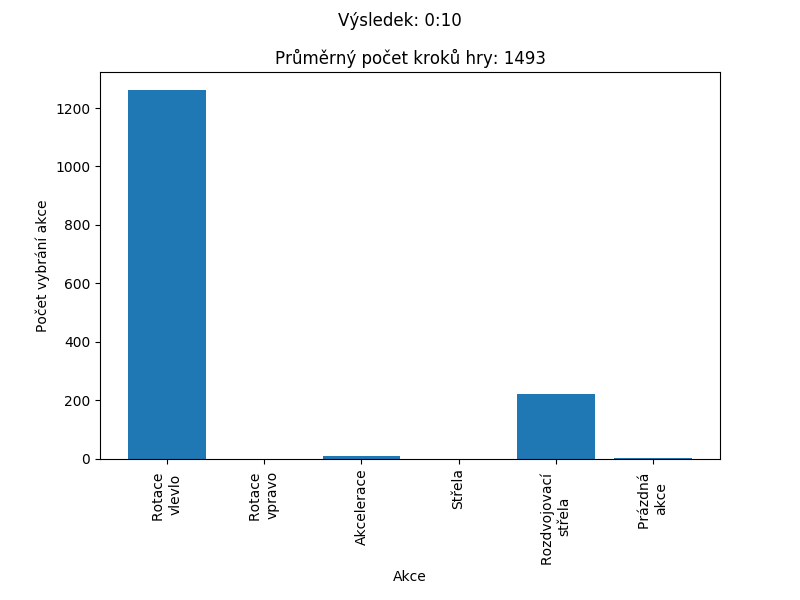
\includegraphics[width=145mm, height=110mm]{./Obrazky/Experiment06Results.png}
\caption{Výsledek experimentu 6}
\label{Výsledek experimentu 06}
\end{figure}
    



\subsection{Experiment 7: Dva elementární agenti}
Tento experiment rozšiřuje experiment předchozí. Budeme opět pracovat s elementárním agentem reprezentovaným neuronovou sítí stejného formátu jako v předhozím případě.
Tentokrát ale nebudeme při trénování hrát hry proti obrannému agentovi, nýbrž proti dalšímu elementárnímu agentovi, který bude také zároveň trénován.
Budeme tedy provádět dvojí q-učení simultánně. Cílem je zde dosáhnout vzájemného adaptivního učení, kde se každý z agentů snaží zlepšovat proti svému nepříteli a postupně tak oba agenty zlepšovat.
\par


Parametry experimentu:
\begin{itemize}
    \item \todo{sjednotit odmeny a penalizaci}
    \item Každý agent bude reprezentován vlastní q-sítí stejného formátu jako v předchozím experimentu.
    \item Tím, že pro souboj nebudeme používat obranného agenta, ale dalšího elementárního agenta, ušetříme čas na výpočtu obranného agenta. V rámci trénování tedy zahrajeme 20000 her.  
    \item Konstanta pro snižoání epsilon je nastavena na hodnotu 0.9998
    \item V posledních 5\% her se nebude epsilon-hladový přístup používat a budou se volit nejlepší známé akce.
\end{itemize}


\begin{figure}[p]\centering
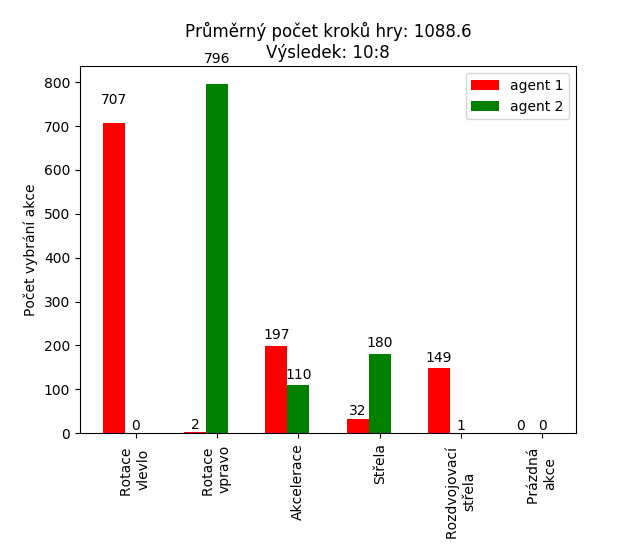
\includegraphics[width=145mm, height=110mm]{./Obrazky/Experiment07Results.png}
\caption{Výsledek experimentu 7}
\label{Výsledek experimentu 07}
\end{figure}


Výsledný souboj jsme výjmečně neprovedli proti obrannému agentovi, ale mezi vzniklými agenty mezi sebou.
Z přehledu souboje je vidět, že se agenti od předchozího experimentu nijak zásadně nezlepšili. Oba agenti se v drtivé většině stavů jen točí na jednu stranu.
Vidíme, že každý agent volí exklusivně pouze jednu stranu, na kterou se rotuje. 
Agent 1 se z přehledu souboje zdá být mírně pestřejší, kombinuje oba typy střel a navíc v téměř pětině stavů volil akceleraci.
Když jsem však vizuálně sledoval souboj agentů, tak žádný z agentů nejevil známky komplexnějšího chování. 